\documentclass[a4paper,12pt]{article}
\usepackage[a4paper,top=1.3cm,bottom=2cm,left=1.5cm,right=1.5cm,marginparwidth=0.75cm]{geometry}
\usepackage{cmap}
\usepackage{mathtext}
\usepackage[T2A]{fontenc}
\usepackage[utf8]{inputenc}
\usepackage[english,russian]{babel}
\usepackage{siunitx}
\usepackage{enumitem}
\usepackage{placeins}

\usepackage{graphicx}
\usepackage{subcaption}
\usepackage{amsmath}

\usepackage{wrapfig}
\usepackage{tabularx}
\usepackage{multirow}

\usepackage{hyperref}
\usepackage[rgb]{xcolor}
\hypersetup{colorlinks=true,urlcolor=blue}
\usepackage{siunitx}
\usepackage{amsmath,amsfonts,amssymb,amsthm,mathtools}
\usepackage{mathtools}
\usepackage{icomma}
\mathtoolsset{showonlyrefs=false}
\usepackage{euscript}
\usepackage{mathrsfs}
\DeclareMathOperator{\sgn}{\mathop{sgn}}
\newcommand*{\hm}[1]{#1\nobreak\discretionary{}
{\hbox{$\mathsurround=0pt #1$}}{}}

%%% Заголовок
\newcommand\labname{Усилитель на биполярных транзисторах}
\newcommand\labnumber{}


\author{Макаров Лев Евгеньевич}
\title{Лабораторная работа №\labnumber

\labname
}

\date{\today}

\makeatletter
\AddEnumerateCounter{\asbuk}{\russian@asbuk@alph}{щ} % section 8.1
\makeatother

\begin{document}

\begin{titlepage}
	\begin{center}
		{\large МОСКОВСКИЙ ФИЗИКО-ТЕХНИЧЕСКИЙ ИНСТИТУТ (НАЦИОНАЛЬНЫЙ ИССЛЕДОВАТЕЛЬСКИЙ УНИВЕРСИТЕТ)}
	\end{center}
	\begin{center}
		{\large Физтех-школа фотоники, электроники и молекулярной физики}
	\end{center}
	
	
	\vspace{4.5cm}
	{\huge
		\begin{center}
			{\bf Отчёт о выполнении лабораторной работы \labnumber}\\
			\labname
		\end{center}
	}
	\vspace{2cm}
	\begin{flushright}
		{\LARGE Автор:\\ Макаров Лев Евгеньевич \\
			\vspace{0.2cm}
			Б04-306}
	\end{flushright}
	\vspace{8cm}
	\begin{center}
		Долгопрудный 2026
	\end{center}
\end{titlepage}

\section{Введение}


\textbf{Цель работы:} собрать усилитель сигнала на биполярных транзисторах; собрать стабилизированную версию; исследовать раюоту усилителя при наличии нагрузки.

\section{Выполнение работы}

\subsection*{Нестабилизированный усилитель}

\begin{enumerate}
    \item Соберем нестабилизированный усилитель согласно схеме на рис. \ref{pic:ustan_1}
\end{enumerate}

\begin{figure}[h]
    \begin{center}
        
\includegraphics[width = 0.35\textwidth]{pictures/ustan_1.png}
        \caption{Схема нестабилизированного усилителя}
    \label{pic:ustan_1}
    \end{center}
\end{figure}

В данном эксперименте $U_\text{П} = 10.68~\text{В}$. Подберем сопротивления так, чтобы ток через коллектор $I_\text{К}$ был приблизительно 5 мА. Так же необходимо вычислить параметр $h_{21}$ для транзистора.

В этой части эксперимента было три итерации установки, отличающиеся напряжением источника $\varepsilon$ и сопротивлениями $R_\text{Б}$ и $R_\text{К}$. Измерения для них представлены в таблице \ref{table:1}.

Напряжения $U_\text{БЭ}$ и $U_\text{КЭ}$ измеряются через модуль ADC на генераторе. Токи вычисляются как

\begin{equation*}
    I_\text{К} = \frac{\varepsilon - U_\text{КЭ}}{R_\text{К}}
\end{equation*}
\begin{equation*}
    I_\text{Б} = \frac{\varepsilon - U_\text{БЭ}}{R_\text{Б}}
\end{equation*}

\begin{table}[!ht]
    \centering
    \caption{\textit{Измерения для нестабилизированного усилителя}}
    \begin{tabular}{l|l|l|l|l|l|l|l|l}
        \hline
          & $\varepsilon$ & $R_\text{Б}$, кОм   & $R_\text{К}$, кОм  & $U_\text{КЭ}$, В & $U_\text{БЭ}$, В & $I_\text{К}$, мА & $I_\text{Б}$, мкА & $h_{21}$ \\ \hline
        1 & 10.68      & 200    & 1     & 7.4   & 0.7   & 3.3  & 49.9 & 66    \\
        2 & 9.99       & 180.15 & 0.590 & 6.05  & 0.69  & 6.67 & 51.6 & 129   \\
        3 & 9.99       & 272.5  & 1.074 & 6.25  & 0.685 & 3.5  & 34.1 & 102   \\ \hline
    \end{tabular}
    \label{table:1}
\end{table}

\clearpage

\begin{enumerate}[resume]
    \item Добавим к усилителю источник колебаний, с сопротивлением и конденсатором согласно схеме на рис. \ref{pic:ustan_2}. Параметры установки представлены в таблице \ref{table:param-2}.
\end{enumerate}

\begin{table}[!ht]
    \centering
    \caption{\textit{Параметры нестабилизированного усилителя с источником}}
    \begin{tabular}{l|l|l|l|l}
        \hline
        $\varepsilon$ & $R_\text{Б}$, кОм   & $R_\text{К}$, кОм & $R_\text{и}$, кОм & $C_\text{Б}$, мкФ  \\ \hline
        9.99      & 219.6    & 1.075 & 1.050 & 220   \\ \hline
    \end{tabular}
    \label{table:param-2}
\end{table}

\begin{figure}[h]
    \begin{center}
        
\includegraphics[width = 0.35\textwidth]{pictures/ustan_2.png}
        \caption{Схема нестабилизированного усилителя с источником колебаний}
    \label{pic:ustan_2}
    \end{center}
\end{figure}

Подберем действующее значение на источнике так, чтобы сигнал, измеряемый осциллографом не искажался: $\widehat{U}_{\text{вых макс}} = 0.12 ~ \text{В}$. Дальнейшие измерения проводились при $\widehat{U} = 0.10~\text{В}$.

Измерим зависимость коэффициентов усиления от частоты входного сигнала:

\begin{equation*}
    K_u = \frac{|A_{out}|}{|A_{in}|}, \ \ \ \ \ K_e = \frac{|A_{out}|}{|\widehat{U}|}
\end{equation*}

Результаты измерений запишем в таблицу \ref{table:2}

\begin{table}[!ht]
    \centering
    \caption{\textit{Измерения коэффициентов усиления}}
    \begin{tabular}{l|r|r|r|r|r}
         & $f$, кГц & $A_{in}$, мВ & $A_{out}$, мВ & $K_u$ & $K_e$ \\ \hline
        0 & 10 & 37 & 7200 & 195 & 72 \\
        1 & 5 & 38 & 6960 & 183 & 70 \\
        2 & 3 & 38 & 6880 & 181 & 69 \\
        3 & 1 & 38 & 6830 & 180 & 68 \\
        4 & 0 & 38 & 6740 & 177 & 67 \\
        5 & 0 & 38 & 6630 & 176 & 66 \\
        6 & 50 & 36 & 7360 & 203 & 74 \\
        7 & 100 & 34 & 7010 & 206 & 70 \\
        8 & 1000 & 8 & 1680 & 210 & 17 \\
        9 & 1100 & 8 & 1630 & 206 & 16 \\
        10 & 500 & 15 & 3350 & 218 & 34 \\
        11 & 60 & 36 & 7500 & 207 & 75 \\
        12 & 599 & 13 & 2940 & 221 & 29 \\
        13 & 699 & 12 & 2560 & 221 & 26 \\
        14 & 800 & 10 & 2240 & 224 & 22 \\
        15 & 901 & 9 & 1990 & 224 & 20 \\ \hline
    \end{tabular}
    \label{table:2}
\end{table}

Построим график и изобразим на рис. \ref{graph:2}.

\begin{figure}[h]
    \begin{center}
        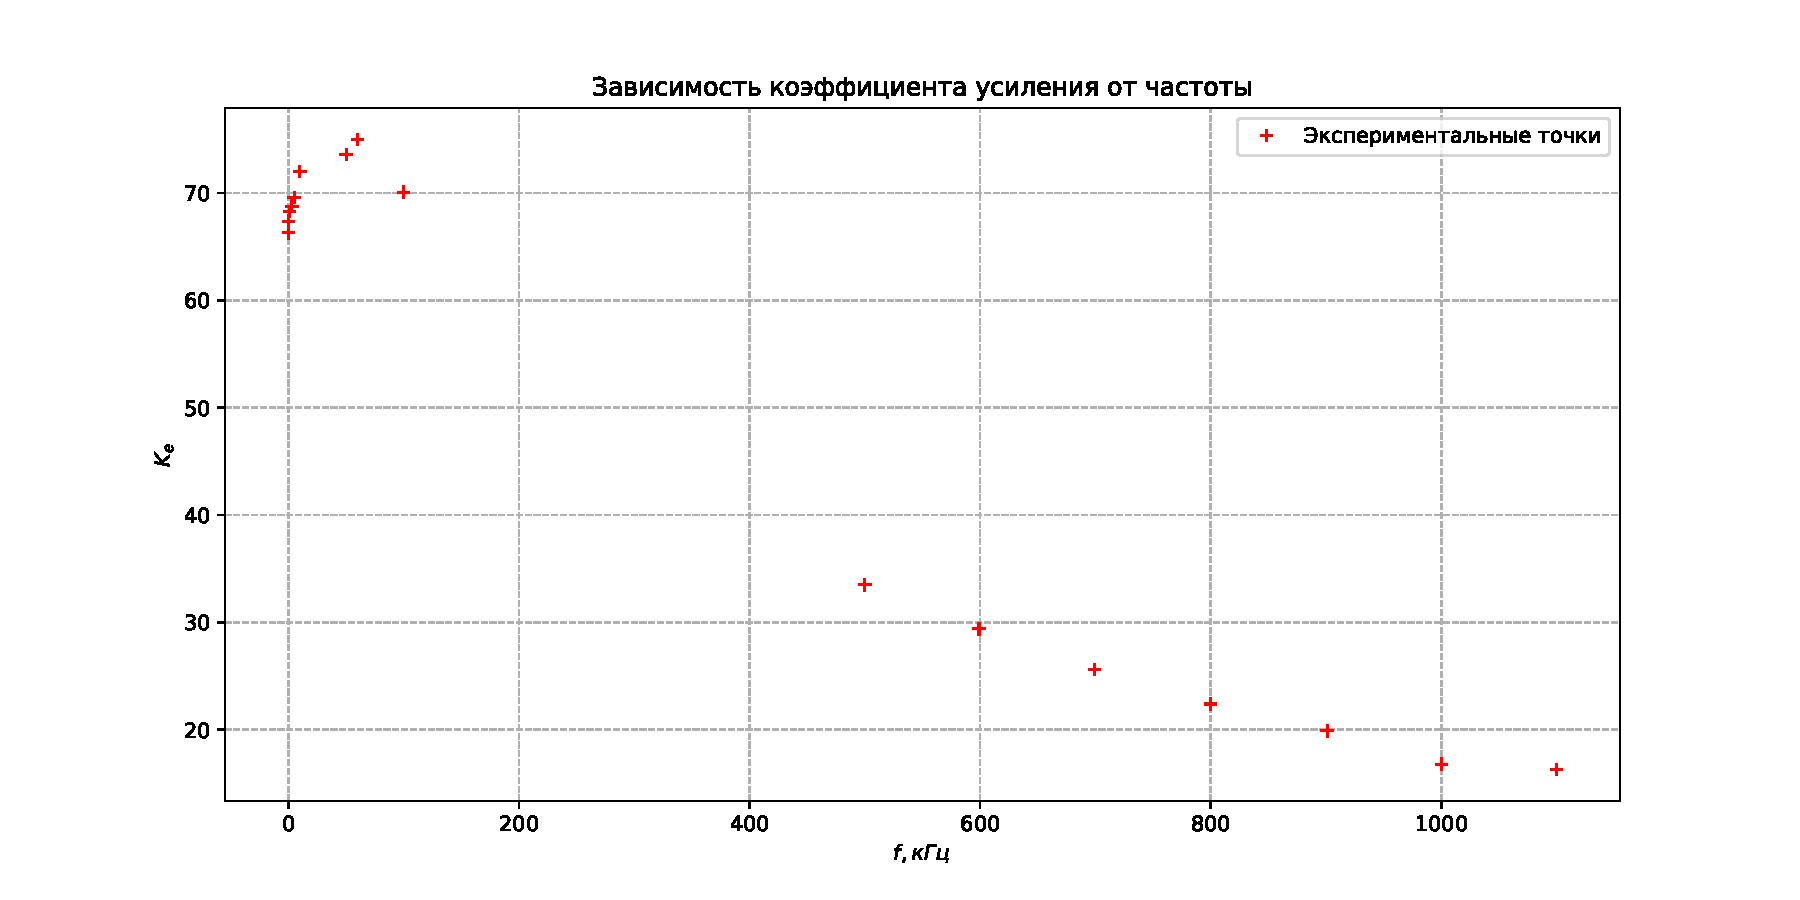
\includegraphics[width=\textwidth]{pictures/graph_2.pdf}
        \caption{Измерение зависимости коэффициента усиления от частоты сигнала источника}
        \label{graph:2}
    \end{center}
\end{figure}

По полученным данным не выходит определить $f_\text{Н}$ и $f_\text{В}$.

\begin{enumerate}[resume]
    \item Добавим к усилителю внешнюю нагрузку $R_\text{Н} \approx R_\text{К}$. Схема изображена на рис. \ref{pic:ustan_3}, параметры установки представлены в таблице \ref{table:param-3}.
\end{enumerate}

\begin{table}[!ht]
    \centering
    \caption{\textit{Параметры нестабилизированного усилителя с источником}}
    \begin{tabular}{l|l|l|l|l|l|l}
        \hline
        $\varepsilon$ & $R_\text{Б}$, кОм   & $R_\text{К}$, кОм & $R_\text{и}$, кОм & $C_\text{Б}$, мкФ &  $R_\text{Н}$, кОм & $C_\text{р}$, мкФ \\ \hline
        9.99 & 187.9 & 1.065 & 1.080 & 220 & 1.065 & 220  \\ \hline
    \end{tabular}
    \label{table:param-3}
\end{table}

\begin{figure}[h]
    \begin{center}
        
\includegraphics[width = 0.35\textwidth]{pictures/ustan_3.png}
        \caption{Схема нестабилизированного усилителя с источником колебаний при подключенной нагрузке}
    \label{pic:ustan_3}
    \end{center}
\end{figure}

Проведем аналогичные измерения предыдущему пункту:

\begin{equation*}
    \widehat{U}_{\text{вых макс}} = 0.12 ~ \text{В}
\end{equation*}

Измерять будем при $\widehat{U} = 0.04~\text{В}$. Результаты измерений запишем в таблицу \ref{table:3}.


\begin{table}[!ht]
    \centering
    \caption{\textit{Измерения коэффициентов усиления при наличии нагрузки}}
    \begin{tabular}{l|r|r|r|r|r}
         & $f$, кГц & $A_{in}$, мВ & $A_{out}$, мВ & $K_u$ & $K_e$ \\ \hline
        0 & 100 & 25 & 3000 & 120 & 75 \\
        1 & 10 & 26 & 2970 & 114 & 74 \\
        2 & 5 & 26 & 2910 & 112 & 73 \\
        3 & 2 & 26 & 3100 & 119 & 78 \\
        4 & 25 & 25 & 3310 & 132 & 83 \\
        5 & 200 & 22 & 3030 & 138 & 76 \\
        6 & 250 & 22 & 2870 & 133 & 72 \\
        7 & 300 & 20 & 2700 & 135 & 68 \\
        8 & 350 & 18 & 2540 & 137 & 64 \\
        9 & 400 & 18 & 2380 & 136 & 60 \\
        10 & 50 & 25 & 3330 & 132 & 83 \\
        11 & 20 & 26 & 3290 & 128 & 82 \\
        12 & 1 & 26 & 3070 & 118 & 77 \\
        13 & 500 & 15 & 2090 & 139 & 52 \\ \hline
    \end{tabular}
    \label{table:3}
\end{table}


Изобразим полученные данные на графике на рис. \ref{graph:3}. По этим измерениям также найдем частоты $f_\text{Н}$ и $f_\text{В}$, при которых коэффициент $K_e$ уменьшается в $\sqrt{2}$ раз.


\begin{figure}[h]
    \begin{center}
        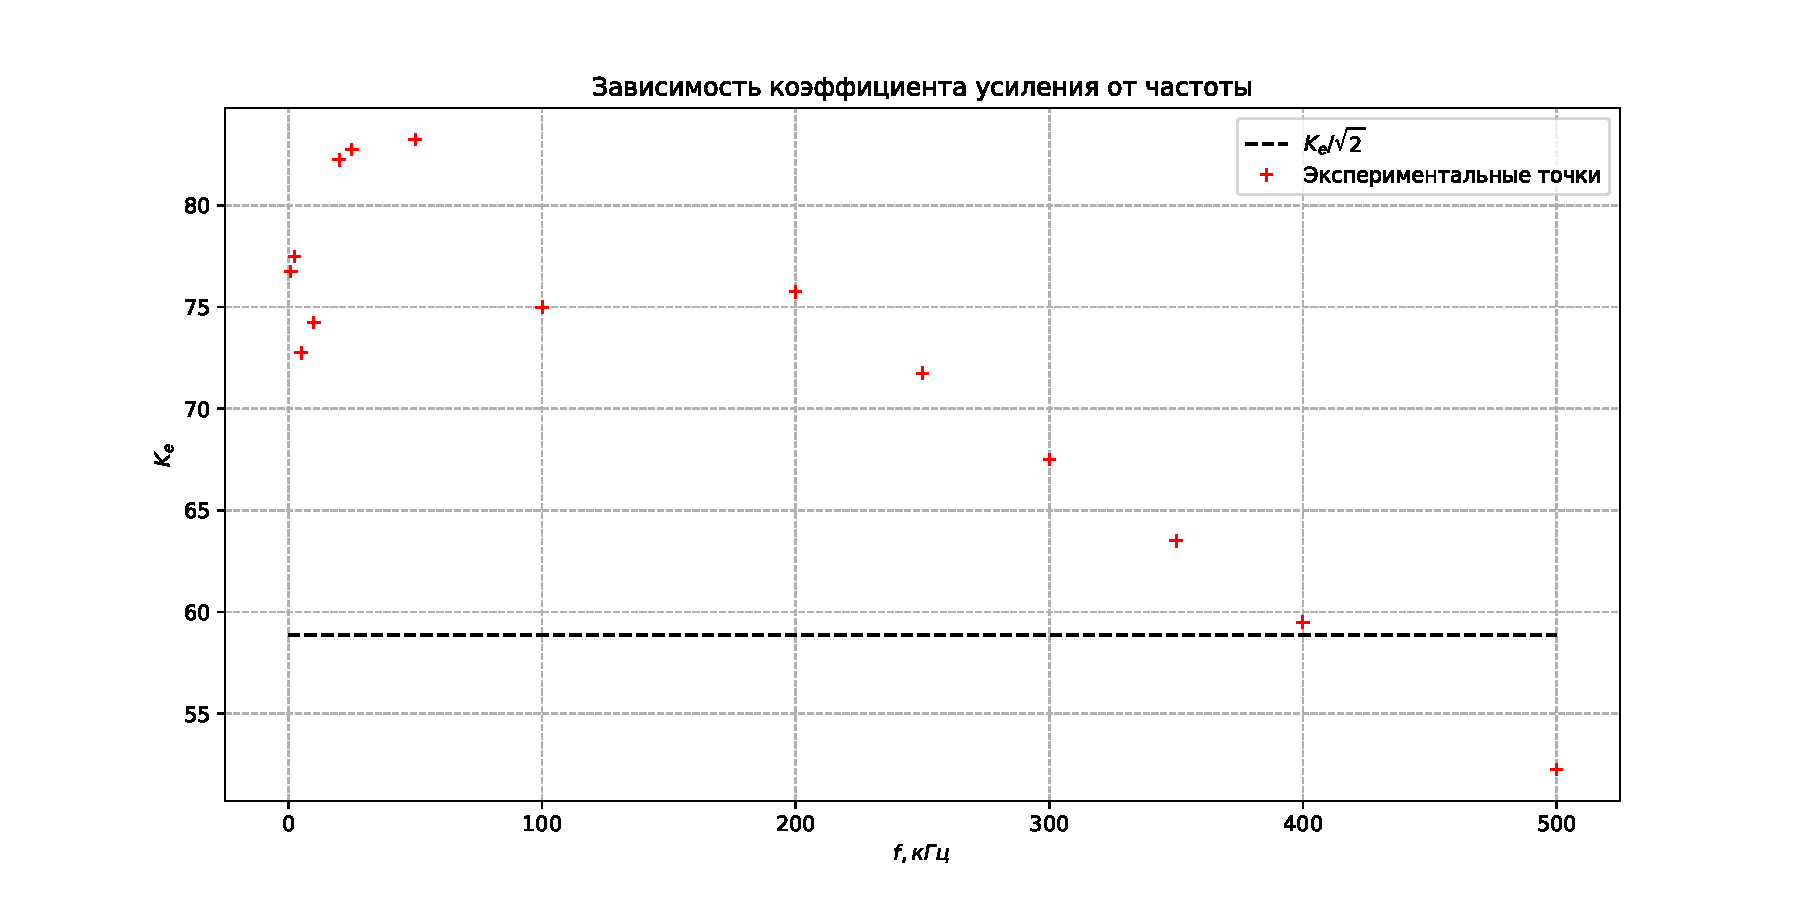
\includegraphics[width=\textwidth]{pictures/graph_3.pdf}
        \caption{Измерение зависимости коэффициента усиления от частоты сигнала источника при наличии нагрузки}
        \label{graph:3}
    \end{center}
\end{figure}

По полученным данным можно оценить $f_\text{В} \approx 400~\text{кГц}$.

\FloatBarrier

\subsection*{Стабилизированный усилитель}

\begin{enumerate}[resume]
    \item Соберем стабилизированный усилитель согласно схеме на рис. \ref{pic:ustan_4}. Параметры указаны в таблице \ref{table:param-4}, представлено несколько итераций установки при подборе оптимальных сопротивлений. Так же там представлены измерения для требуемых напряжений и вычисление тока $I_\text{К}$
\end{enumerate}

\begin{figure}[h]
    \begin{center}
        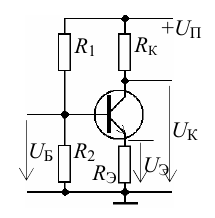
\includegraphics[width = 0.35\textwidth]{pictures/ustan_4.png}
        \caption{Схема стабилизированного усилителя}
    \label{pic:ustan_4}
    \end{center}
\end{figure}

\begin{table}[!ht]
    \centering
    \caption{\textit{Параметры стабилизированного усилителя}}
    \begin{tabular}{l|l|l|l|l|l|l|l|l}
        \hline
        $\varepsilon$ & $R_1$, кОм   & $R_\text{К}$, кОм & $R_2$, кОм & $R_\text{Э}$, Ом & $U_\text{Б}$, В & $U_\text{Э}$, В & $U_\text{К}$, В & $I_\text{К}$, мА \\ \hline
        9.99 & 0.4699 & 1.065 & 1.999 & 269.4 & 9.09 & 1.9  & 9.3  & 7.05 \\ \hline
        9.99 & 0.747  & 1.065 & 1.999 & 269.4 & 8.5  & 1.47 & 8.8  & 5.4  \\ \hline
        9.99 & 11.1   & 1.065 & 1.999 & 269.4 & 4.22 & 1.6  & 5.02 & 4.6  \\ \hline
    \end{tabular}
    \label{table:param-4}
\end{table}

При дальнейших измерениях была использована последняя итерация.

\begin{enumerate}[resume]
    \item Добавим конденсатор к эмиттеру и подключим источник согласно схеме на рис. \ref{pic:ustan_5}, параметры установки указаны в таблице \ref{pic:ustan_5}
\end{enumerate}

\begin{figure}[h]
    \begin{center}
        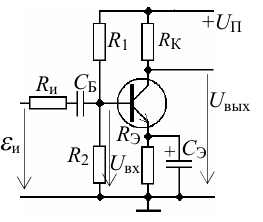
\includegraphics[width = 0.35\textwidth]{pictures/ustan_5.png}
        \caption{Схема стабилизированного усилителя с источником и емкостью на эмиттере}
    \label{pic:ustan_5}
    \end{center}
\end{figure}

\begin{table}[!ht]
    \centering
    \caption{\textit{Параметры стабилизированного усилителя}}
    \begin{tabular}{l|l|l|l|l|l|l|l}
        \hline
        $\varepsilon$ & $R_1$, кОм   & $R_\text{К}$, кОм & $R_2$, кОм & $R_\text{Э}$, Ом & $R_\text{и}$, кОм & $C_\text{Б}$, мкФ & $C_\text{Э}$, мкФ \\ \hline
        9.99 & 11.1   & 1.065 & 1.999 & 269.4 & 1.080 & 220 & 220  \\ \hline
    \end{tabular}
    \label{table:param-4}
\end{table}

Далее проведем измерения предельных частот при $\widehat{U} = 0.222~ \text{в}$. Результаты измерений запишем в таблицу \ref{table:5}

\begin{table}[!ht]
    \centering
    \caption{\textit{Измерения коэффициентов усиления для стабилизированного усилителя}}
    \begin{tabular}{l|r|r|r|r|r}
         & $f$, кГц & $A_{in}$, мВ & $A_{out}$, мВ & $K_u$ & $K_e$ \\ \hline
        0 & 100 & 82 & 4900 & 60 & 22 \\
        1 & 20 & 85 & 7030 & 83 & 32 \\
        2 & 200 & 78 & 4360 & 56 & 20 \\
        3 & 300 & 74 & 4111 & 56 & 19 \\
        4 & 50 & 83 & 5990 & 72 & 27 \\
        5 & 10 & 85 & 6500 & 76 & 29 \\
        6 & 1 & 87 & 7200 & 83 & 32 \\ \hline
    \end{tabular}
    \label{table:5}
\end{table}


Изобразим полученные данные на графике на рис. \ref{graph:5}. По этим измерениям также найдем частоты $f_\text{Н}$ и $f_\text{В}$, при которых коэффициент $K_e$ уменьшается в $\sqrt{2}$ раз.


\begin{figure}[!ht]
    \begin{center}
        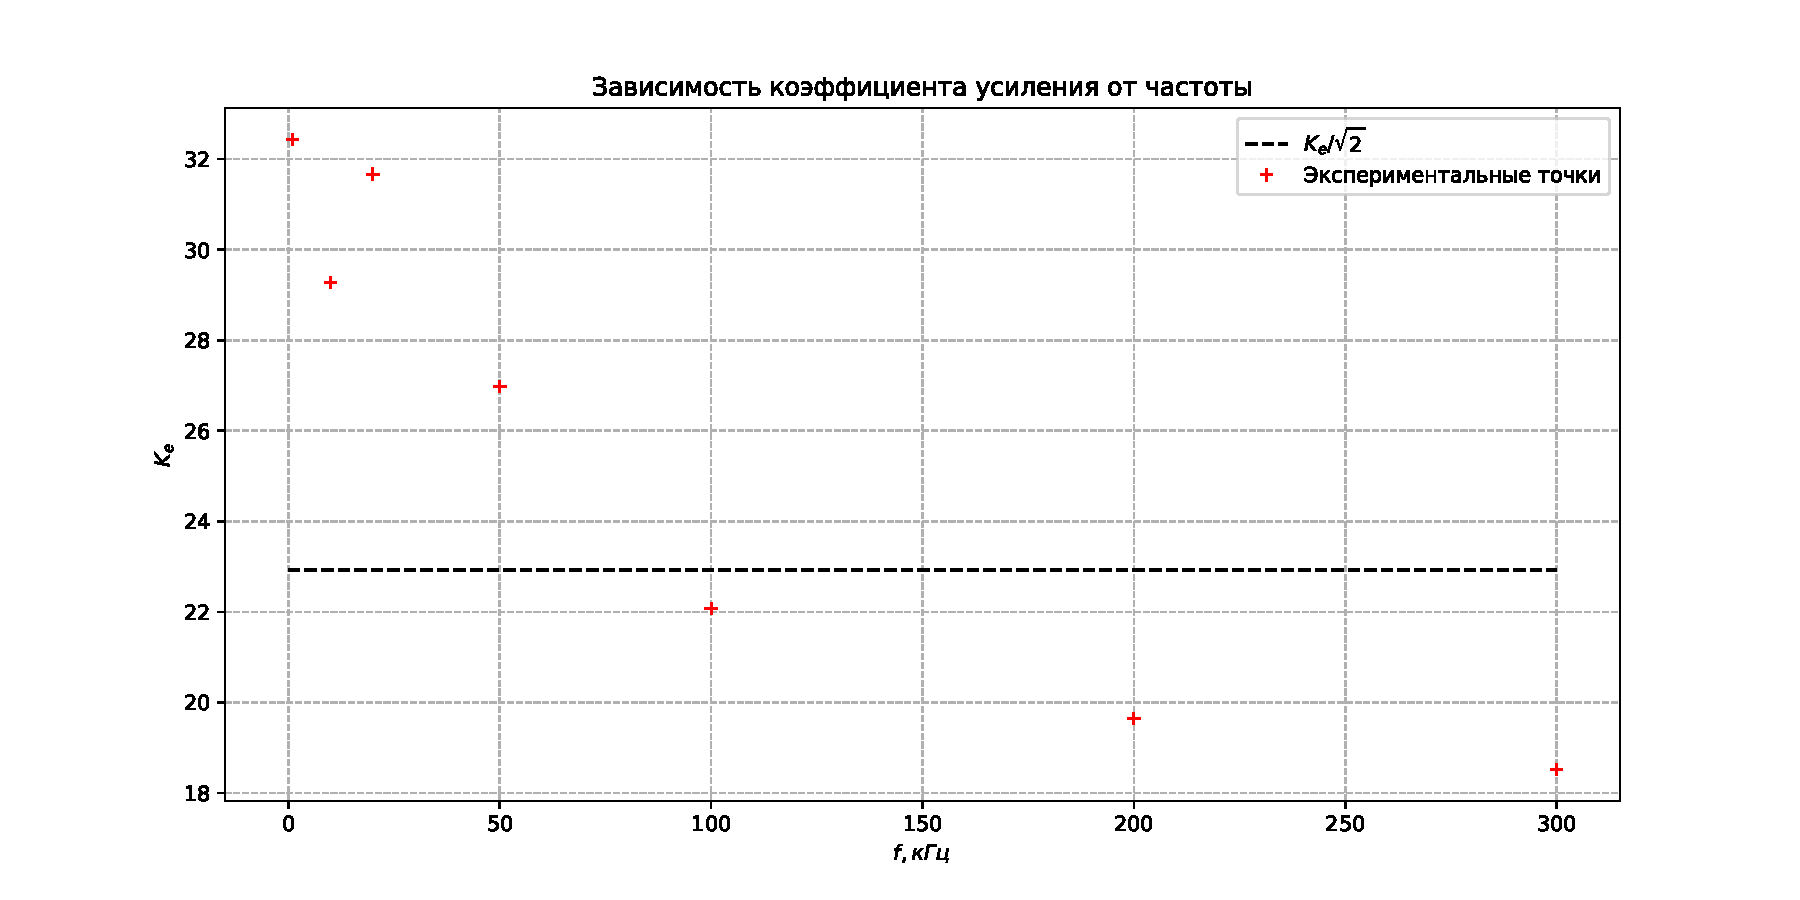
\includegraphics[width=\textwidth]{pictures/graph_5.pdf}
        \caption{Измерение зависимости коэффициента усиления от частоты сигнала источника для стабилизированного усилителя}
        \label{graph:5}
    \end{center}
\end{figure}

По полученным данным можно оценить $f_\text{В} \approx 80~\text{кГц}$.

\begin{enumerate}[resume]
    \item Подадим на усилитель прямоугольный сигнал ширины $T = 5 / 2\pi f_\text{В} \approx 8 ~ \text{мкс}$. По осциллографу измерим ширину импульса на выходе $\tau_\text{В} = 23.7 - 19.6 = 4.1 ~ \text{мкс}$.
    \item Уберем емкость эмиттера и проведем измерения частот. Схема установки в этом случае на рис. \ref{pic:ustan_7}. Параметры установки в таблице \ref{table:param-7}.
\end{enumerate}

\begin{figure}[h]
    \begin{center}
        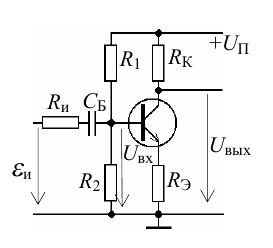
\includegraphics[width = 0.35\textwidth]{pictures/ustan_7.png}
        \caption{Схема стабилизированного усилителя с источником без емкости на эмиттере}
    \label{pic:ustan_7}
    \end{center}
\end{figure}

\begin{table}[!ht]
    \centering
    \caption{\textit{Параметры стабилизированного усилителя без емкости на эмиттере}}
    \begin{tabular}{l|l|l|l|l|l|l|l}
        \hline
        $\varepsilon$ & $R_1$, кОм   & $R_\text{К}$, кОм & $R_2$, кОм & $R_\text{Э}$, Ом & $R_\text{и}$, кОм & $C_\text{Б}$, мкФ \\ \hline
        9.99 & 11.1   & 1.065 & 1.999 & 269.4 & 1.080 & 220  \\ \hline
    \end{tabular}
    \label{table:param-7}
\end{table}

Далее проведем измерения предельных частот при $\widehat{U} = 0.1~ \text{в}$. Результаты измерений запишем в таблицу \ref{table:7}

\begin{table}[!ht]
    \centering
    \caption{\textit{Измерения коэффициентов усиления для стабилизированного усилителя без емкости на эмиттере}}
    \begin{tabular}{l|r|r|r|r|r}
         & $f$, кГц & $A_{in}$, мВ & $A_{out}$, мВ & $K_u$ & $K_e$ \\ \hline
        0 & 300 & 57 & 1180 & 21 & 12 \\
        1 & 200 & 58 & 1220 & 21 & 12 \\
        2 & 100 & 58 & 1350 & 23 & 14 \\
        3 & 10 & 58 & 2210 & 38 & 22 \\
        4 & 50 & 57 & 1600 & 28 & 16 \\
        5 & 5 & 59 & 2260 & 38 & 23 \\
        6 & 40 & 58 & 1740 & 30 & 17 \\
        7 & 30 & 58 & 1890 & 33 & 19 \\
        8 & 20 & 58 & 2050 & 35 & 20 \\ \hline
    \end{tabular}
    \label{table:7}
\end{table}

Изобразим полученные данные на графике на рис. \ref{graph:7}. По этим измерениям также найдем частоты $f_\text{Н}$ и $f_\text{В}$, при которых коэффициент $K_e$ уменьшается в $\sqrt{2}$ раз.


\begin{figure}[!ht]
    \begin{center}
        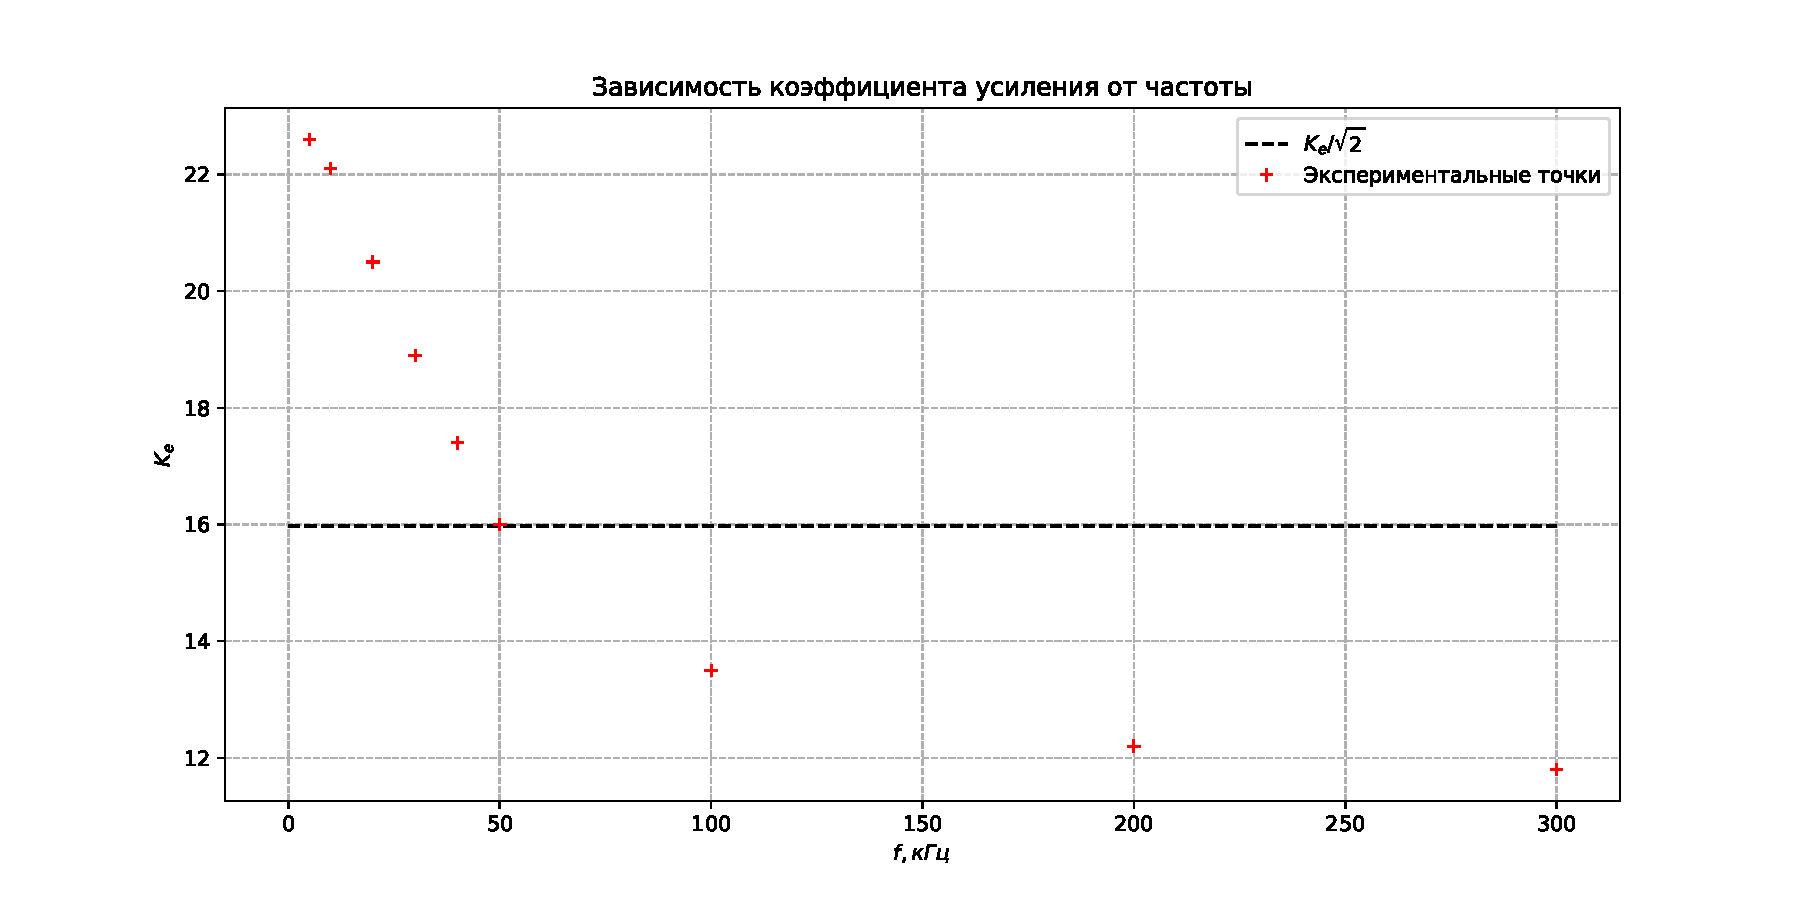
\includegraphics[width=\textwidth]{pictures/graph_7.pdf}
        \caption{Измерение зависимости коэффициента усиления от частоты сигнала источника для стабилизированного усилителя без емкости на эмиттере}
        \label{graph:7}
    \end{center}
\end{figure}

По полученным данным можно оценить $f_\text{В} \approx 50~\text{кГц}$.

\subsection*{Двухканальный усилитель}

\begin{enumerate}[resume]
    \item Упражнение не выполнялось.
\end{enumerate}



\end{document}
